\documentclass[12pt]{article}

\title{Visualizing the complex Mandelbrot trajectories}
\author{S. Halayka\footnote{sjhalayka@gmail.com}}
\date{\today}

\usepackage{listings}
\usepackage{cite}
\usepackage{xcolor}
\usepackage{graphicx}
\usepackage{setspace}
\usepackage{amsmath}
\usepackage{url}

\usepackage{caption}
\usepackage{subcaption}

%\usepackage[margin=1in]{geometry}
%\doublespace
\begin{document}




\maketitle

\begin{abstract}
The trajectories of the complex Mandelbrot set are visualized using Catmull-Rom curves and OpenGL.
\end{abstract}



\section{What is the complex Mandelbrot set?}

The complex Mandelbrot set is a set of vertices in 2D (complex) space that satisfy a particular mathematical criterion -- the trajectory assocated with each vertex remains within the sphere defined by threshold $= 4$ while undergoing iteration.

See Figure 1 for the visualization of an input grid.
See Figure 2 for the tiny C++ iteration code.
As shown in Figure 2, the iterative equation is
\begin{equation}
Z = Z^2 + C.
\end{equation}

See Figure 3 for a low-resolution version of the Mandelbrot set.

See Figure 4 for a visualization of some of the complex Mandelbrot trajectories.
See Figure 5 for a medium-resolution version of the Mandelbrot set.
See Figure 6 for all of the complex Mandelbrot trajectories.

The primary motivation for the exploration of the trajectories of the complex Mandelbrot set was to introduce a new type of visualization: see Figure 7 for all of the Mandelbrot trajectories, drawn using Catmull-Rom curves using rainbow colouring.


\section{Why Catmull-Rom curves?}

Compared to  B\'ezier curves, Catmull-Rom curves seem to encode a higher degree of fidelity when it comes to the line passing through all of the control points.

Catmull-Rom curves offer $C_1$ continuity -- continuity in both position and tangent vectors.
As such, the closed (periodic) loops of the complex Mandelbrot set are easy to visualize.
On the other hand, B\'ezier curves do not offer such built-in $C_1$ continuity.

See Figure 8 for all of the Mandelbrot trajectories, drawn using Catmull-Rom curves and pseudorandomly-assigned colours.

Catmull-Rom curves are as computationally intensive as B\'ezier curves, but not much more.

Catmull-Rom curves are attractive, in several different ways.

The quaternion Mandelbrot set is also briefly considered in Figure 9.






\begin{thebibliography}{9}
\bibitem{bourke} Bourke. (2018) ``3D volumetric fractal trajectories''
\bibitem{halayka} Halayka. (2018) ``Visualizing the escape paths of quaternion fractals''
\bibitem{chen} Chen. (2017) ``C++ B\'ezier / spline / Catmull-Rom curve library'' \linebreak \url{https://github.com/chen0040/cpp-spline}
\bibitem{ventrella} Ventrella. (2021) ``Mandelbrot Orbits'' JavaScript Web Applet \linebreak \url{http://www.ventrella.com/mandelbrot_orbits/}



\end{thebibliography}



\pagebreak

\begin{figure} 
\centering
  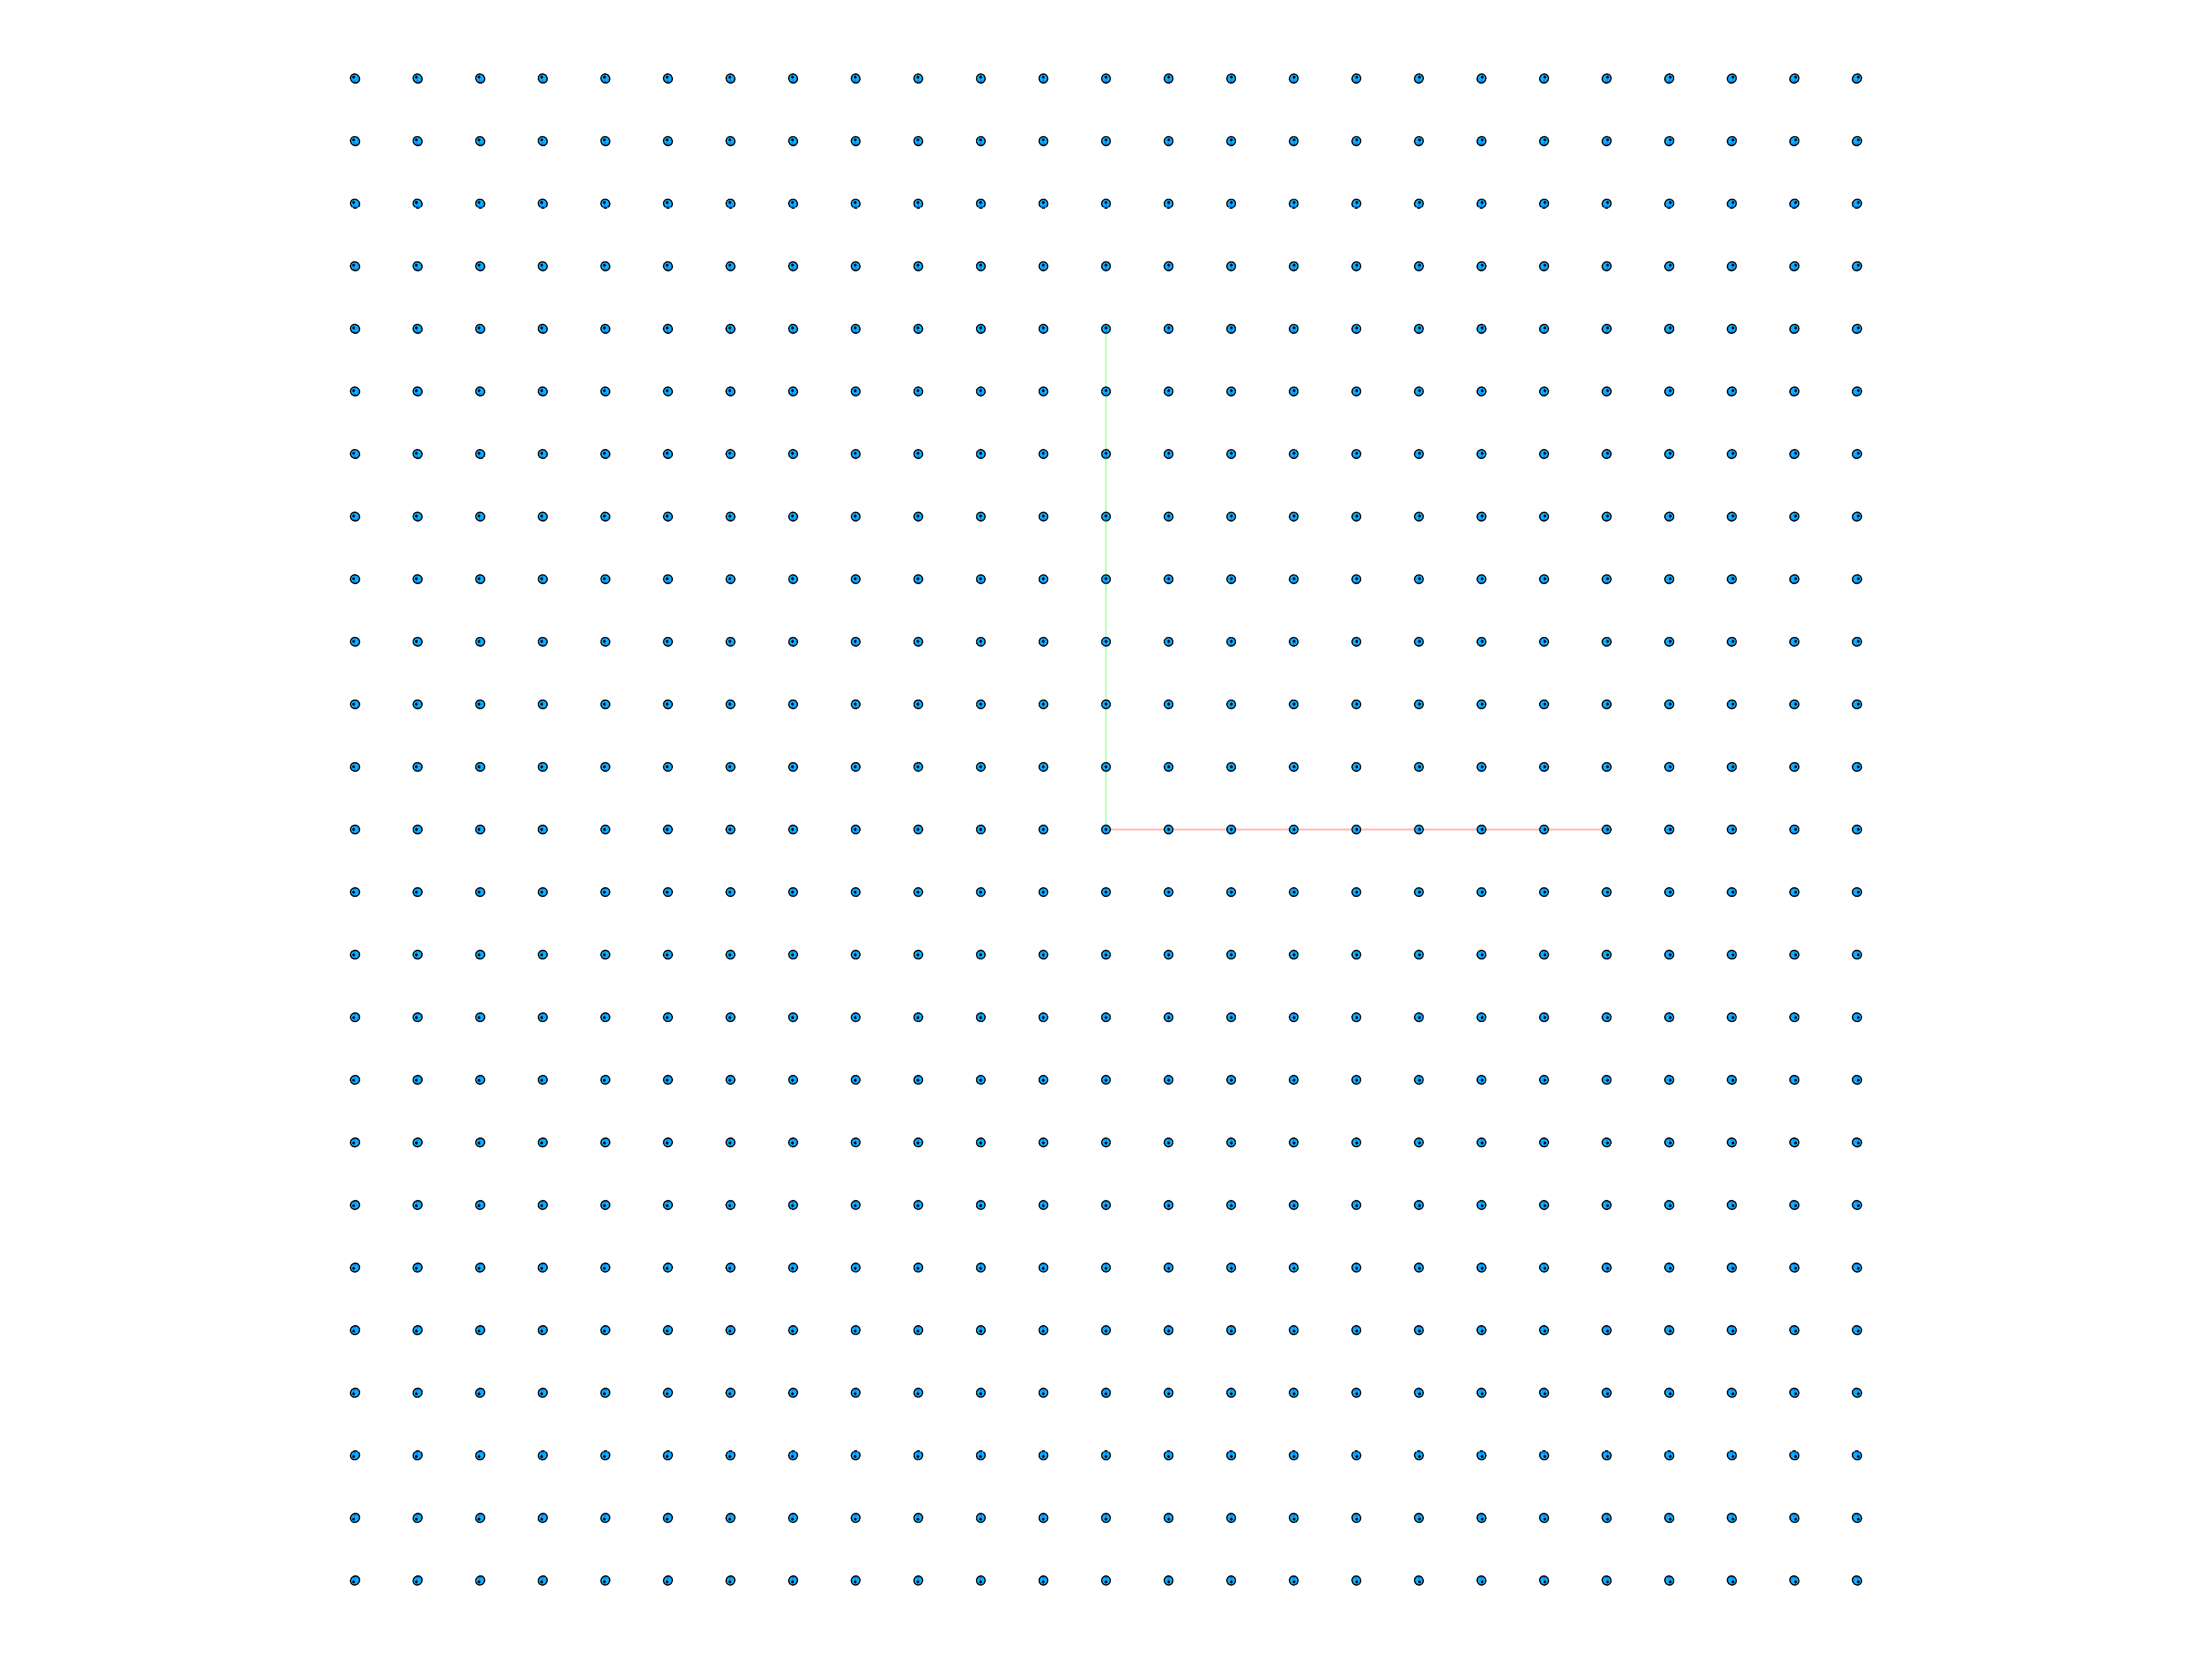
\includegraphics[width = 5 in]{grid.png}	
  \caption{Grid of sample vertices.
Grid minimum = -1.5, grid maximum = 1.5.
Resolution = 25.
}
\end{figure}


\begin{figure} 
\centering
  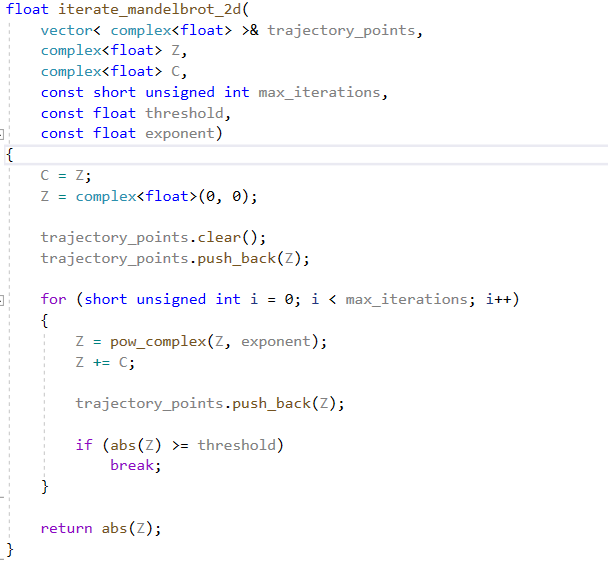
\includegraphics[width = 5 in]{code1.png}	
  \caption{Iteration C++ code.
The exponent is 2 in this paper.
}
\end{figure}

\begin{figure} 
\centering
  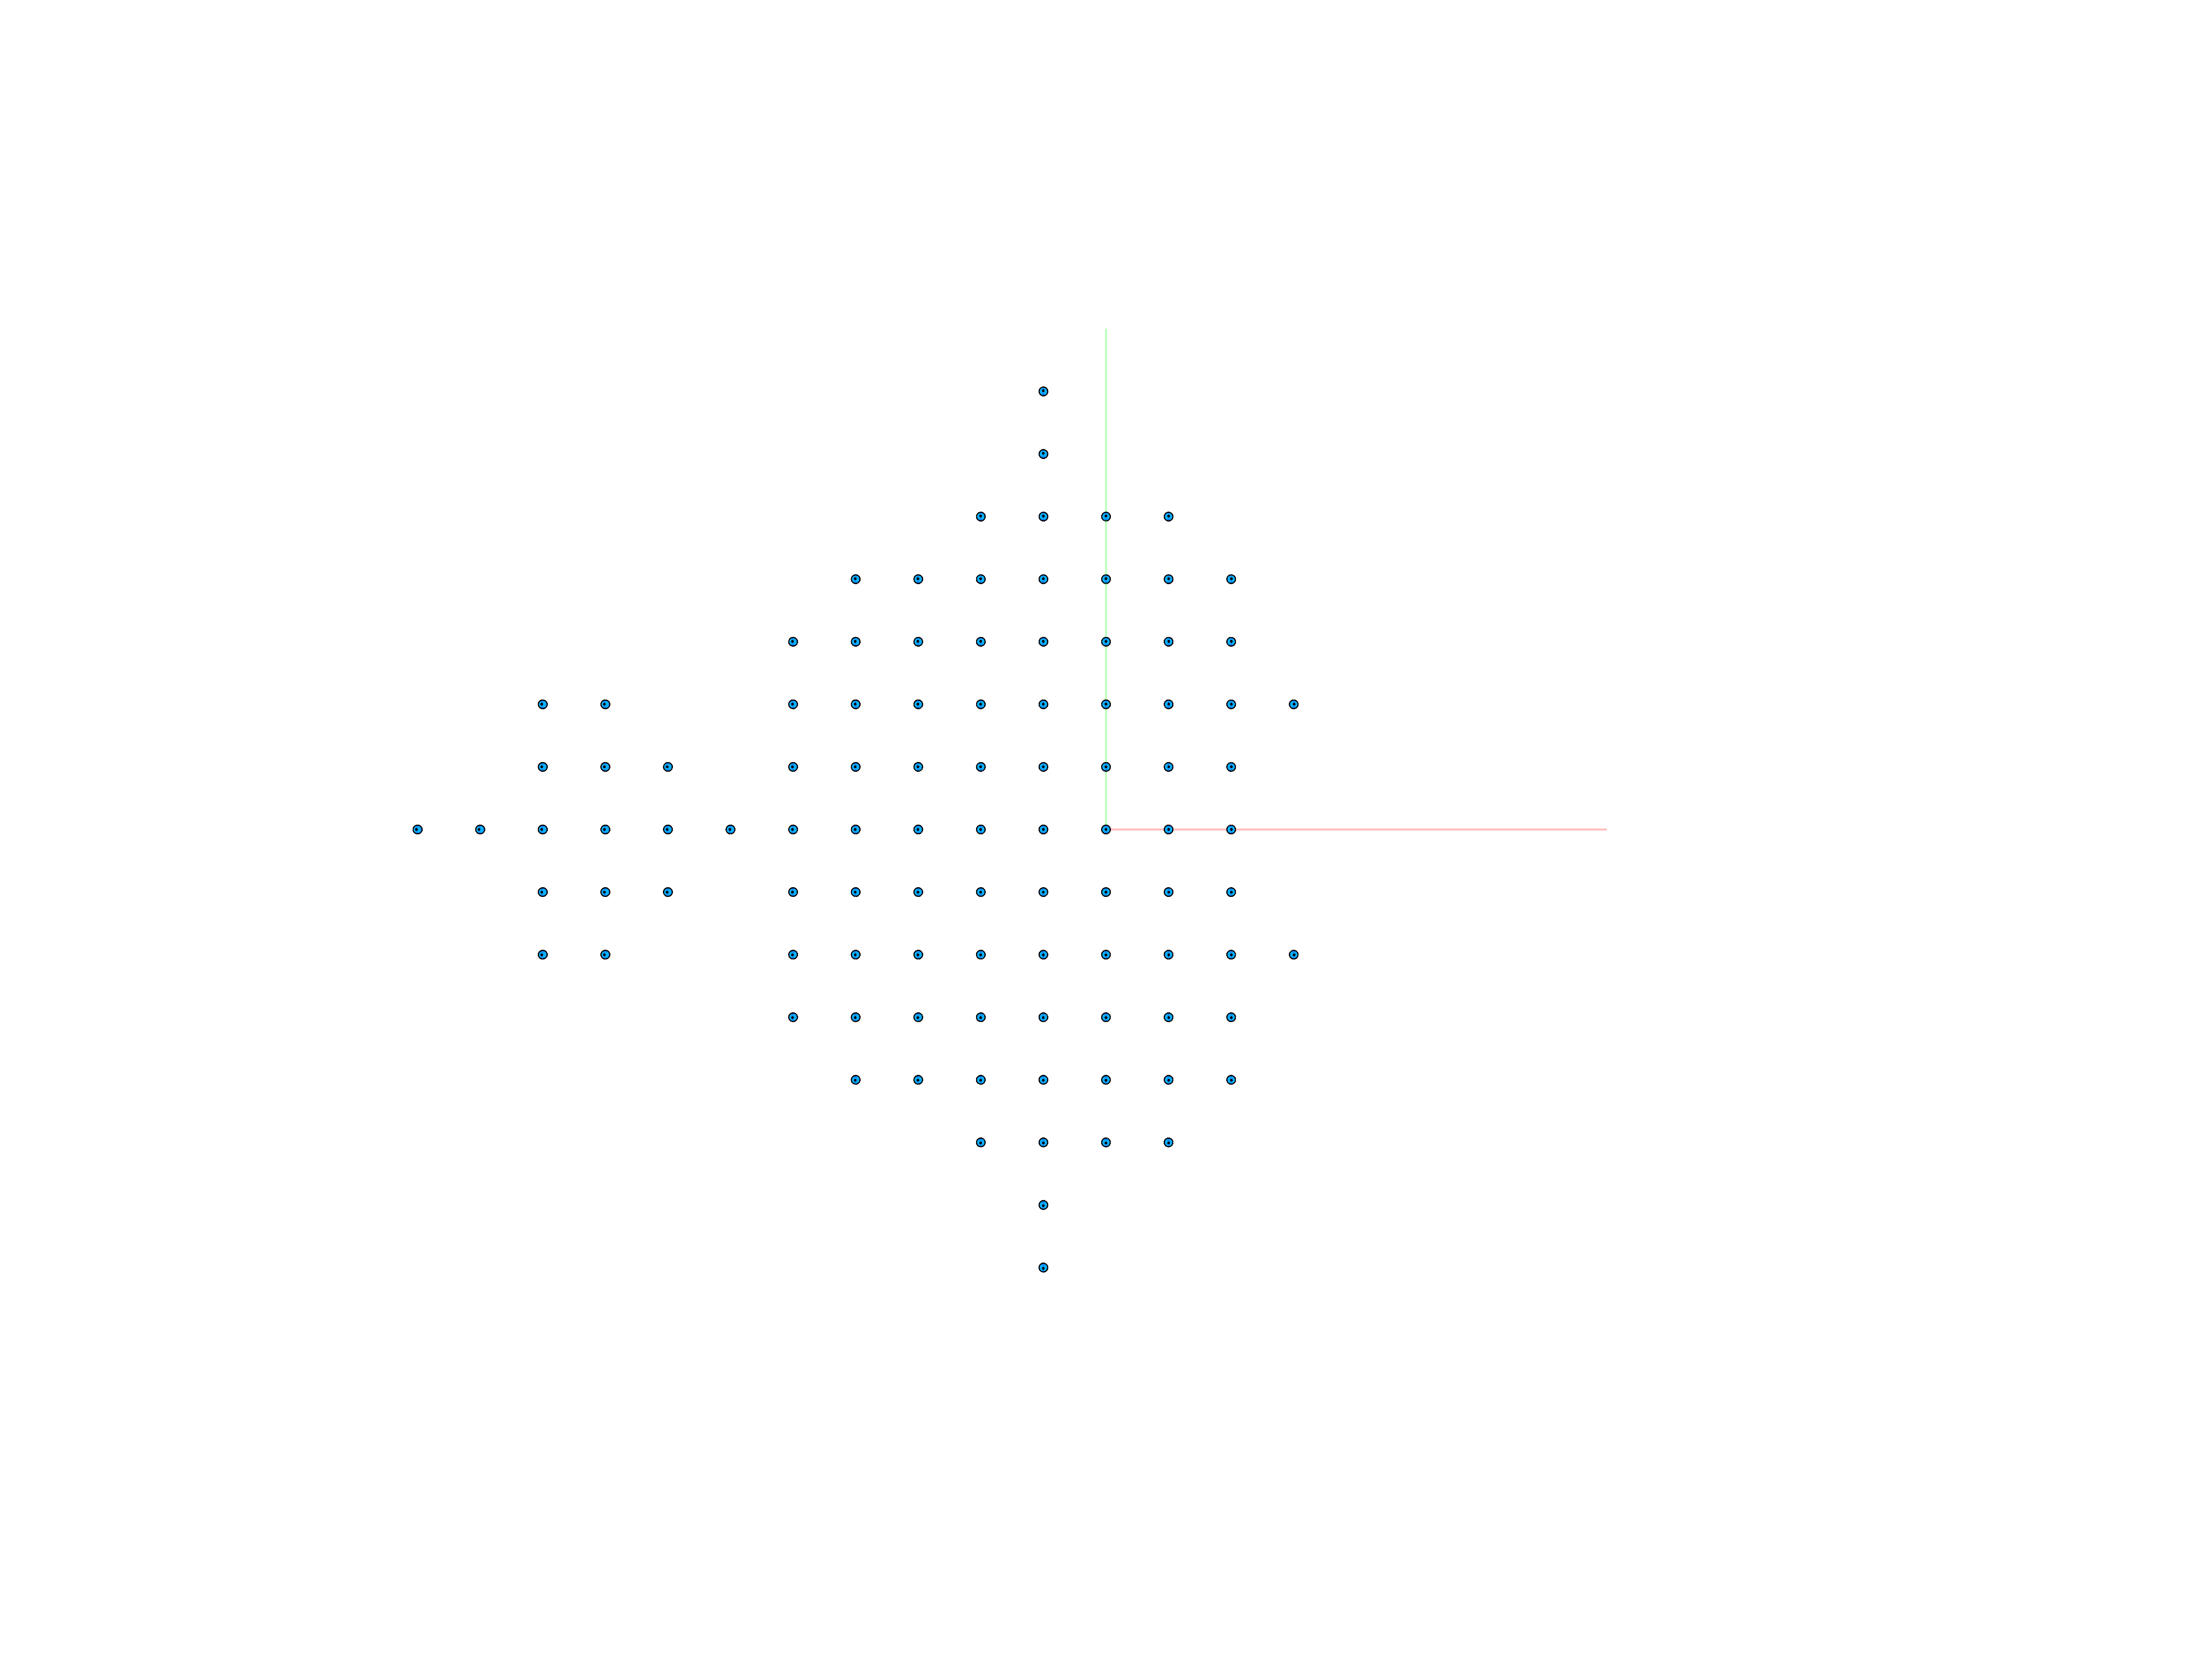
\includegraphics[width = 5 in]{set1.png}	
  \caption{Low-resolution version of the complex Mandelbrot set.
Only the vertices within the set are drawn.
Maximum iterations = 500.
Grid minimum = -1.5, grid maximum = 1.5.
Threshold = 4.0.
Resolution = 25.
}
\end{figure}

\begin{figure} 
\centering
  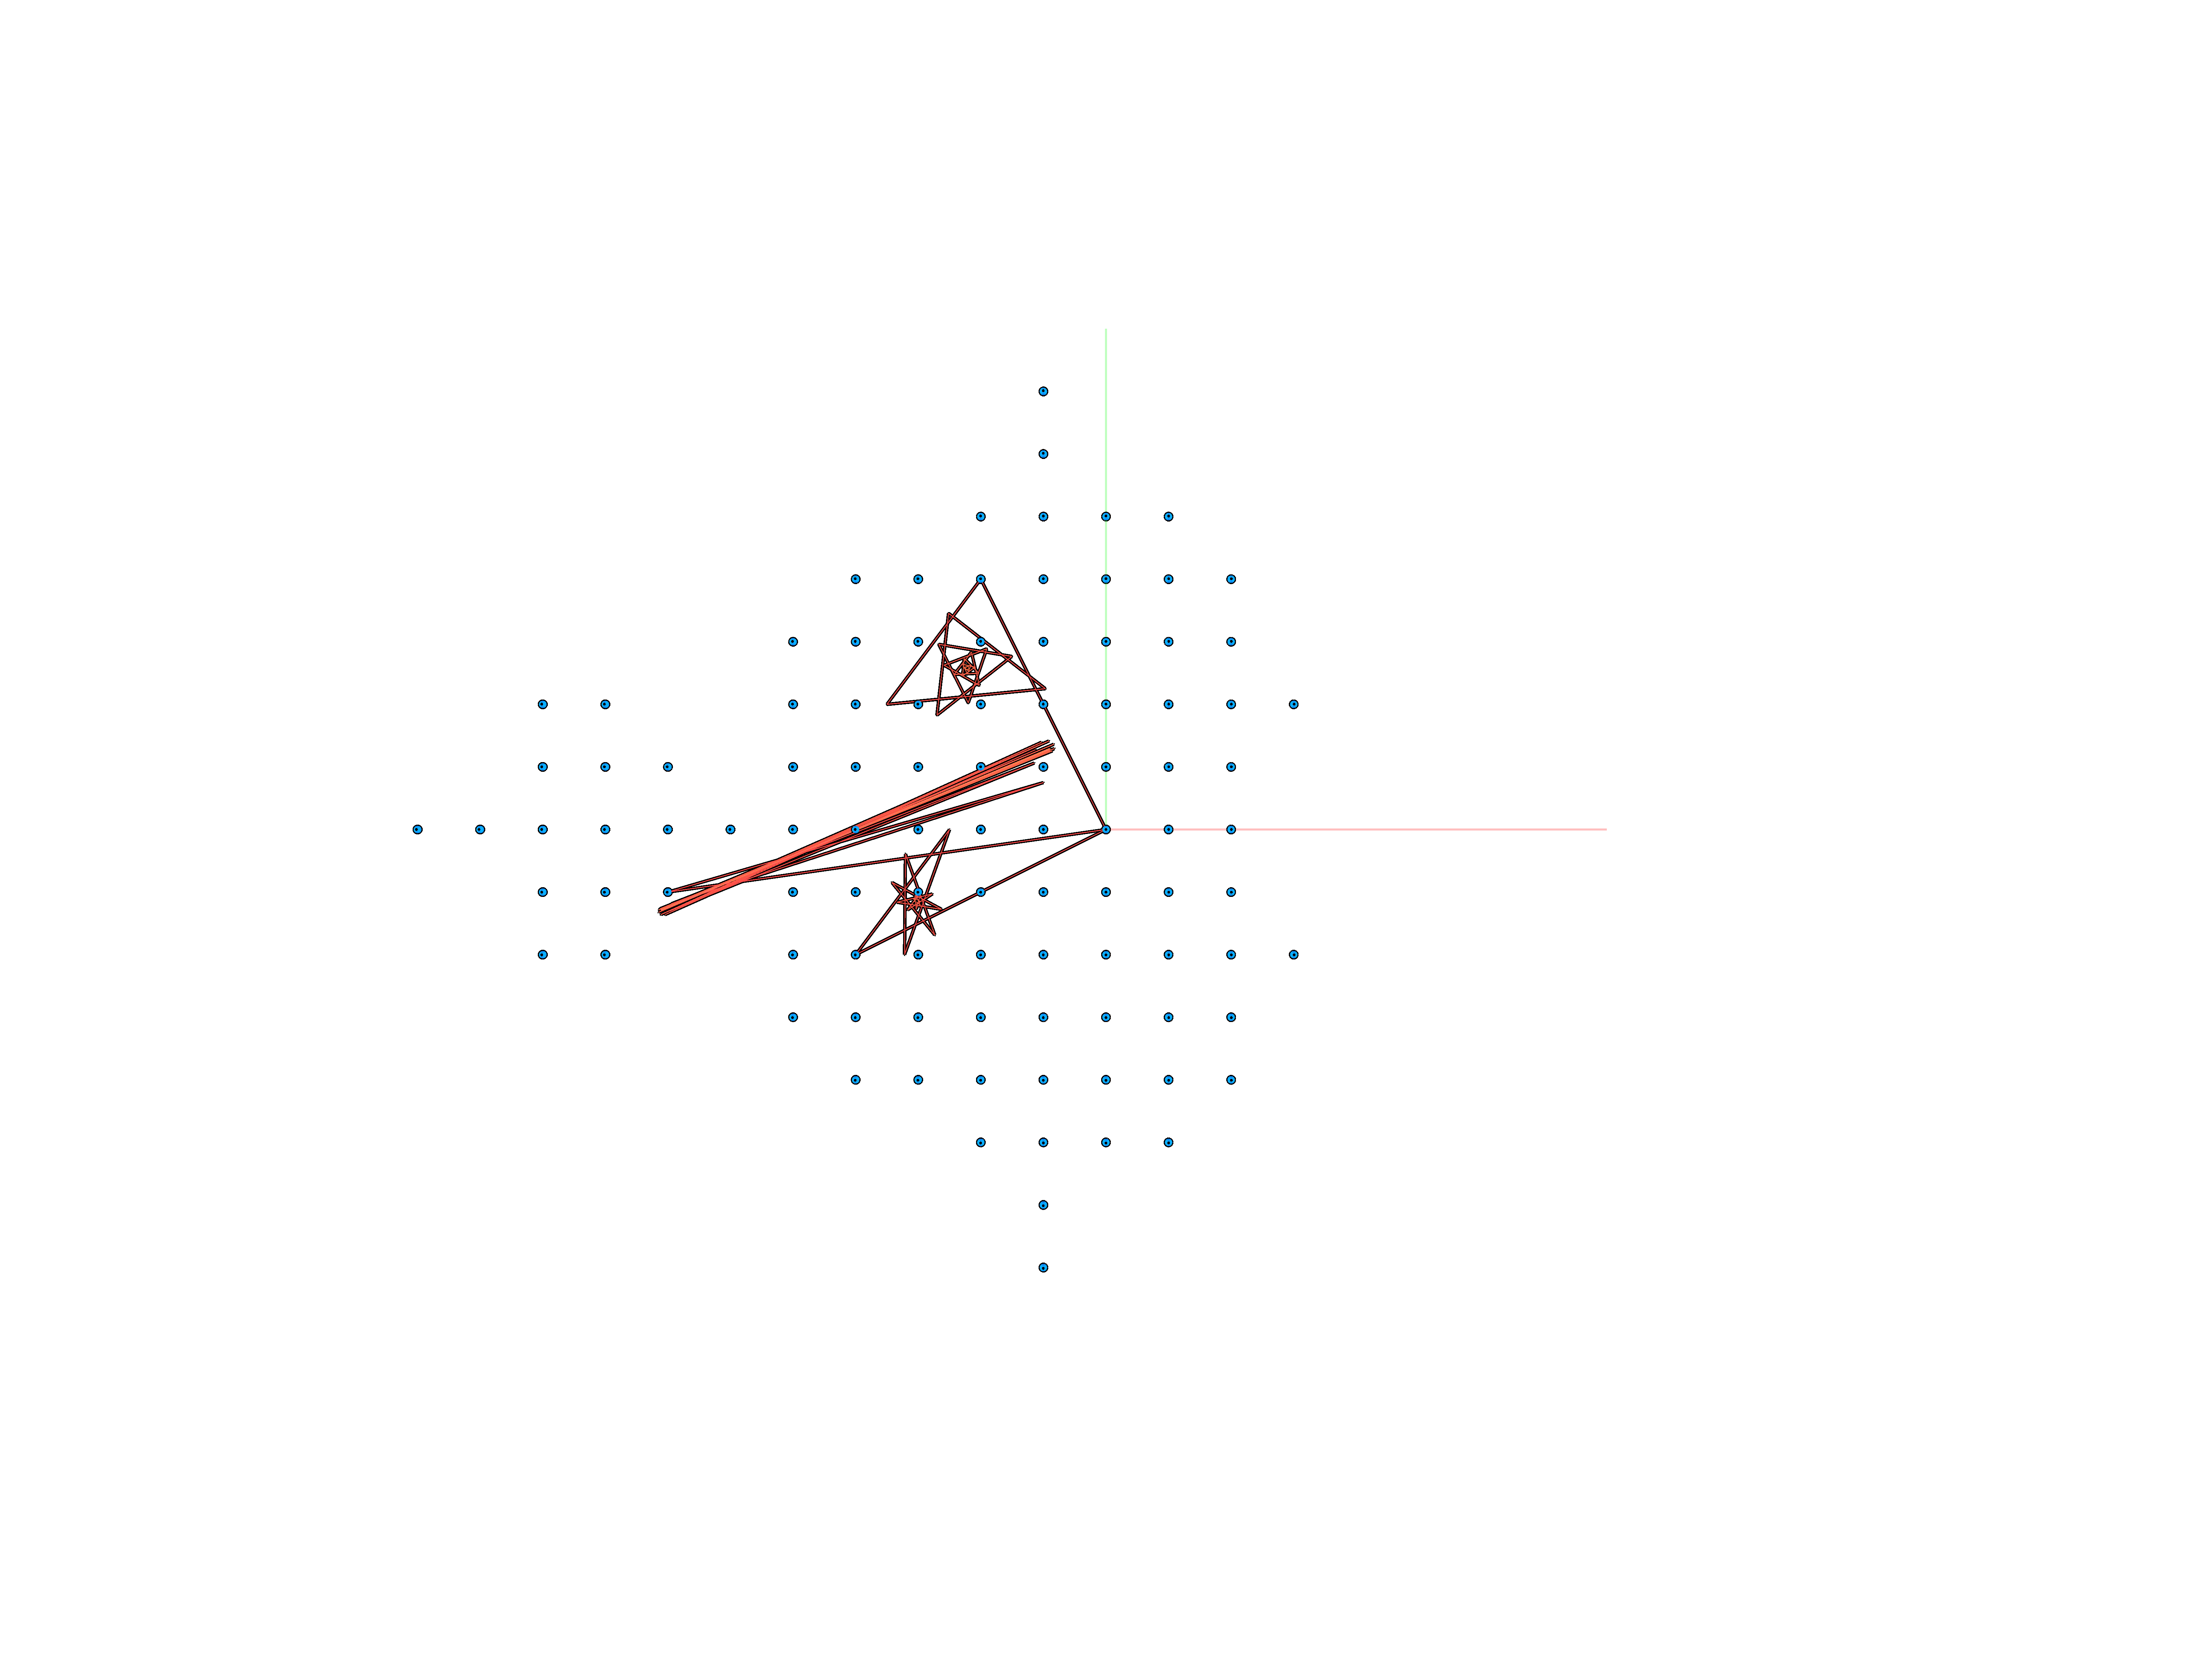
\includegraphics[width = 5 in]{sample_trajectories.png}	
  \caption{A few examples of the complex Mandelbrot trajectories.
Maximum iterations = 500.
Grid minimum = -1.5, grid maximum = 1.5.
Threshold = 4.0.
Resolution = 25.
}
\end{figure}


\begin{figure} 
\centering
  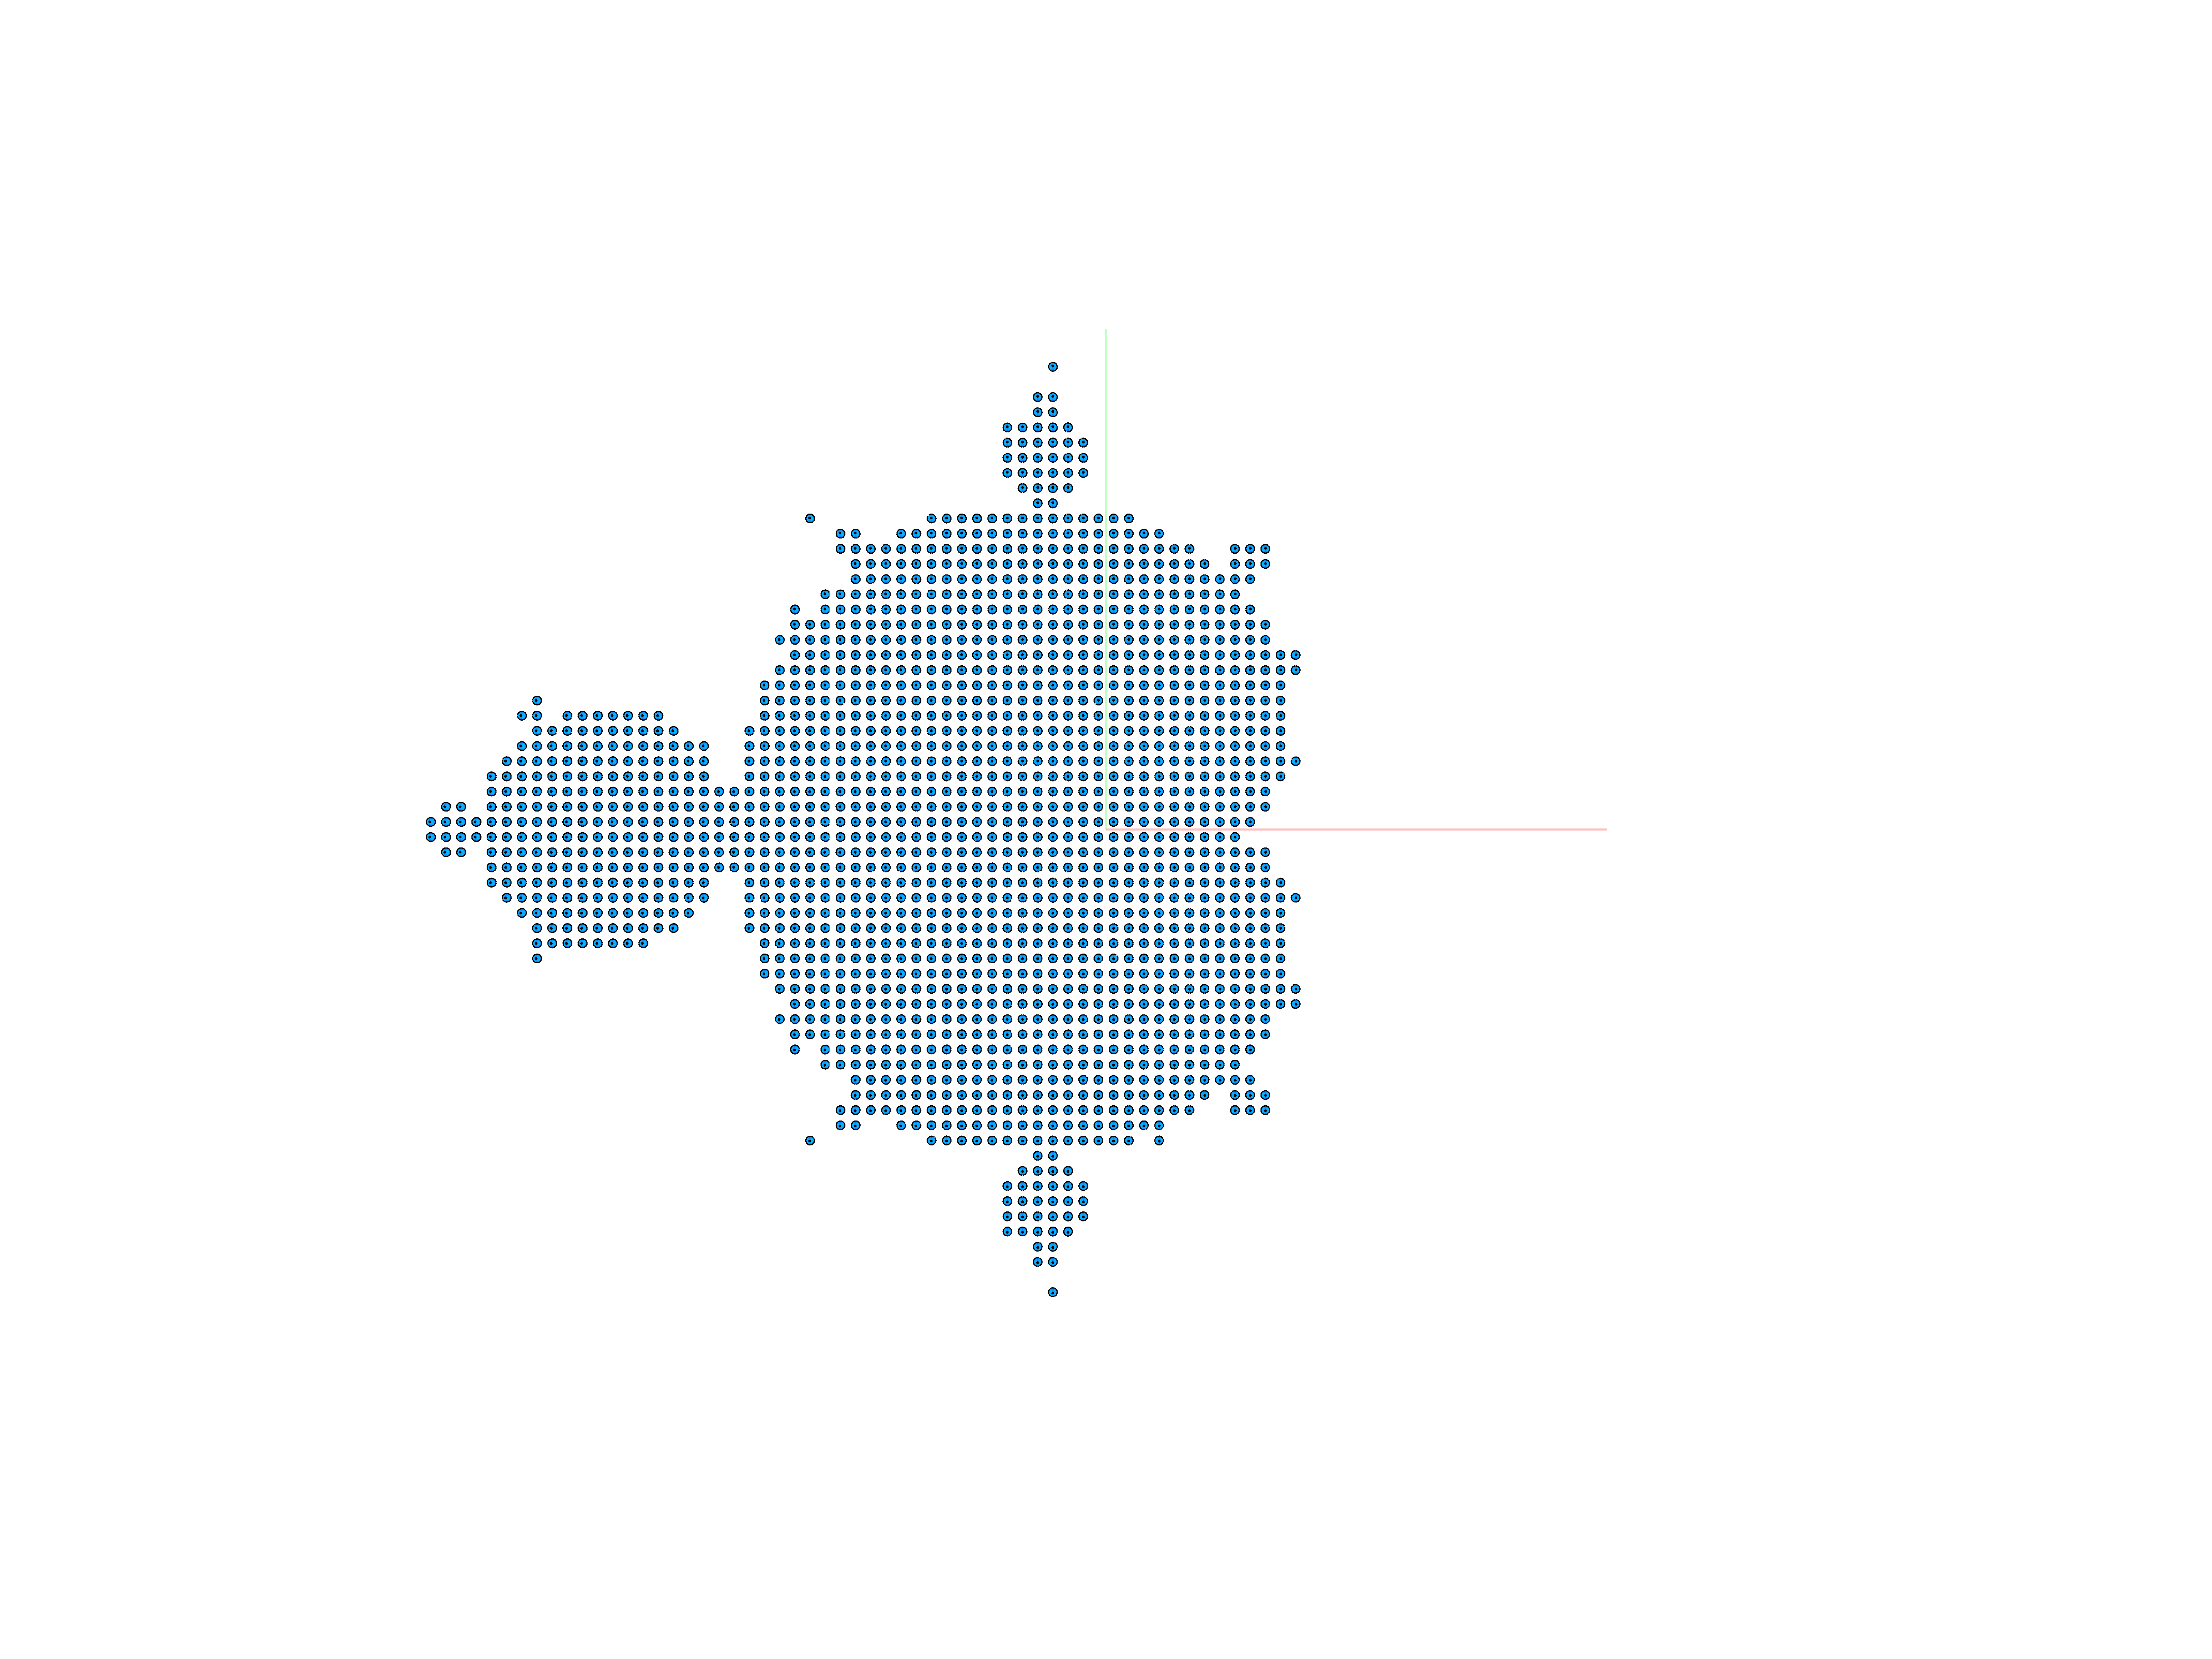
\includegraphics[width = 5 in]{set2.png}	
  \caption{Medium-resolution version of rhe complex Mandelbrot set.
Maximum iterations = 500.
Grid minimum = -1.5, grid maximum = 1.5.
Threshold = 4.0.
Resolution = 100.
}
\end{figure}


\begin{figure} 
\centering
  \includegraphics[width = 6.5 in]{rainbow_500_iterations_non_curved.png}	
  \caption{Complex Mandelbrot set.
Maximum iterations = 500.
Grid minimum = -1.5, grid maximum = 1.5.
Threshold = 4.0.
Resolution = 25.
Actual trajectories are drawn.
The majority of the trajectories end up being periodic orbits.}
\end{figure}


\begin{figure} 
\centering
  \includegraphics[width = 5 in]{rainbow_500_iterations.png}	
  \caption{
Complex Mandelbrot set.
Maximum iterations = 500.
Grid minimum = -1.5, grid maximum = 1.5.
Threshold = 4.0. 
Resolution = 25.
Catmull-Rom trajectories are drawn.
The majority of the trajectories end up being periodic orbits.}
\end{figure}

\begin{figure} 
\centering
  \includegraphics[width = 5 in]{pseudorandom_500_iterations.png}	
  \caption{
Complex Mandelbrot set.
Maximum iterations = 500.
Grid minimum = -1.5, grid maximum = 1.5.
Threshold = 4.0.
Resolution = 25.
Catmull-Rom trajectories are drawn.
Pseudorandomly-assigned colours are used, to help differentiate between the individual trajectories.
The majority of the trajectories end up being periodic orbits.}
\end{figure}










\begin{figure} 
\centering
  \includegraphics[width = 5 in]{quaternion_mandelbrot.png}	
  \caption{
Quaternion Mandelbrot set.
Maximum iterations = 500.
Grid minimum = -1.5, grid maximum = 1.5.
Threshold = 4.0.
Resolution = 10.
Catmull-Rom trajectories are drawn.
As is with the complex Mandelbrot set, the majority of the quaternion Mandelbrot trajectories end up being periodic orbits.}
\end{figure}


\end{document}









